
\documentclass[hyperref={pdfpagelabels=false},ngerman]{beamer}

% stop font warning
\let\Tiny=\tiny
\providecommand\thispdfpagelabel[1]{}

\usepackage[english]{babel}
\usepackage{lmodern}
\usepackage[T1]{fontenc}
\usepackage[utf8]{inputenc}
\usepackage{graphicx,import}
\usepackage{feynmp}
\DeclareGraphicsRule{*}{mps}{*}{} 
\DeclareGraphicsExtensions{.pdf}
\usepackage{amsmath,amssymb,amstext,amsfonts} % mathrsfs
\usepackage{array,booktabs,tabularx}
\usepackage{tikz,tikz-uml,pgf-pie}
\usetikzlibrary{shapes,calc,arrows,positioning}
\tikzstyle{block} = [rectangle, draw, text width=7em, text centered, minimum height=2em]
\tikzstyle{arrow} = [draw, -latex, thick]
\tikzstyle{arrow2} = [draw, latex-latex, thick]
\tikzstyle{quark}  = [rectangle, draw, fill=yellow, minimum width=2em, text centered, minimum height=2em]
\tikzstyle{lepton} = [rectangle, draw, fill=red!50, minimum width=2em, text centered, minimum height=2em]
\tikzstyle{gauge}  = [circle   , draw, fill=green , minimum size=2em, inner sep=0pt, text centered]
\tikzstyle{scalar} = [diamond  , draw, fill=blue!40, minimum width=2.3em, text centered, minimum height=2.3em, inner sep=0pt]
\tikzstyle{goldstone} = [diamond, draw, dashed, fill=blue!30, minimum width=2.3em, text centered, minimum height=2.3em, inner sep=0pt]
\tikzstyle{squark}   = [diamond, draw, fill=yellow, minimum width=2.3em, text centered, minimum height=2.3em, inner sep=0pt]
\tikzstyle{slepton}  = [diamond, draw, fill=red!50, minimum width=2.3em, text centered, minimum height=2.3em, inner sep=0pt]
\tikzstyle{gaugino}  = [rectangle, draw, fill=green , minimum size=2em, inner sep=0pt, text centered]
\tikzstyle{higgsino} = [rectangle, draw, fill=blue!40  , minimum width=2em, text centered, minimum height=2em]
\tikzstyle{inert}    = [diamond  , draw, fill=teal!80, minimum width=2.3em, text centered, minimum height=2.3em, inner sep=0pt]
\tikzstyle{inertino} = [rectangle, draw, fill=teal!80, minimum width=2em, text centered, minimum height=2em]
\tikzstyle{phantom}  = [rectangle, minimum width=2em, text centered, minimum height=2em]
\usepackage{slashed}
\usepackage{fixltx2e} % textsubscript
\usepackage{multirow}
\usepackage{tcolorbox}
\usepackage{pifont}
\usepackage{hyperref}
\hypersetup{colorlinks,linkcolor=,urlcolor=blue}
\usepackage{listings}
\lstset{breaklines=true,
  breakatwhitespace=true,
%  numbers=left,
  numberstyle=\tiny,
  stepnumber=1,
  basicstyle=\ttfamily\footnotesize,
  commentstyle=\ttfamily\color{gray},
  postbreak={\mbox{{$\hookrightarrow$}}\space\space},
  breakindent=10pt,
  breakautoindent=false,
  showspaces=false,
  showstringspaces=false,
  frame=single}

\definecolor{darkgreen}{RGB}{0,176,0}

\newcommand{\cmark}{\ding{51}}%
\newcommand{\xmark}{\ding{55}}%
\newcommand{\fmfvcenter}[1]{\;\vcenter{\hbox{\fmfreuse{#1}}}\;}
\newcommand{\eh}[1]{\,\mathsf{#1}}
\newcommand{\ok}{\textcolor{darkgreen}{\cmark}}
\newcommand{\notok}{\textcolor{red}{\xmark}}
\newcommand{\maybe}{\textcolor{gray}{\cmark}}
\newcommand{\Lagr}{\mathcal{L}}
\newcommand{\mathi}{\mathsf{i}}
\newcommand{\mycite}[1]{\textcolor{darkgray}{\tiny [#1]}}
\newcommand{\bigcite}[1]{\textcolor{darkgray}{[#1]}}
\newcommand{\dimrep}[1]{\mathbf{#1}}
\newcommand{\dimrepadj}[1]{\mathbf{\overline{#1}}}
\newcommand{\ESSM}{E\textsubscript{6}SSM}
\newcommand{\CESSM}{CE\textsubscript{6}SSM}
\DeclareMathOperator{\tildeRe}{\widetilde Re}
\DeclareMathOperator{\sign}{sign}
\DeclareMathOperator{\re}{Re}
\DeclareMathOperator{\im}{Im}
\renewcommand{\emph}{\textbf}
\newcommand{\dd}{\mathsf{d}}
\newcommand{\myurl}[1]{\href{#1}{#1}}
\newcommand{\Superpot}{\mathcal{W}}
\newcommand{\SuperField}[1]{#1}
\newcommand{\ConjSuperField}[1]{\bar{#1}}
\newcommand{\UY}{\ensuremath{U(1)_{Y}}}
\newcommand{\UN}{\ensuremath{U(1)_{N}}}
\newcommand{\Uem}{\ensuremath{U(1)_\text{em}}}
\newcommand{\SUL}{\ensuremath{SU(2)_\text{L}}}
\newcommand{\SUc}{\ensuremath{SU(3)_\text{c}}}
\newcommand{\SOten}{\ensuremath{{SO(10)}}}
\newcommand{\comma}{,}
\newcommand{\DRbar}{\ensuremath{\overline{\text{DR}}}}
\newcommand{\MSbar}{\ensuremath{\overline{\text{MS}}}}
\newcommand{\SM}{\ensuremath{\text{SM}}}
\newcommand{\MSSM}{\ensuremath{\text{MSSM}}}
\newcommand{\pole}{\ensuremath{\text{pole}}}
\newcommand{\tree}{\ensuremath{\text{tree}}}
\newcommand{\Zv}{\ensuremath{\backslash\mkern-11.0mu{Z_3}}}
\newcommand{\downrightknickarrow}{\mathrel{\scalebox{1.3}{\rotatebox[origin=c]{180}{$\Lsh$}}}}
\newcommand{\threelinebrace}{$\left. \begin{array}{c} \\ \\ \\ \end{array} \right\rbrace$}
\newcommand{\fivelinebrace}{$\left. \begin{array}{c} \\ \\ \\ \\ \\ \end{array} \right\rbrace$}
\newcommand{\twolinebrace}{$\left. \begin{array}{c} \\ \\ \end{array} \right\rbrace$}
\newcommand{\elevenlinebrace}{$\left. \begin{array}{c} \\ \\ \\ \\ \\ \\ \\ \\ \\ \\ \\ \end{array} \right\rbrace$}

% set look of slides
\usetheme{Madrid}
\useoutertheme{default}
\useinnertheme{circles}
\usecolortheme{default}
\beamertemplatenavigationsymbolsempty % keine Navigationselemente
\setbeamersize{text margin left = 1cm, text margin right = 1cm}

% define footer
\makeatletter
\setbeamertemplate{footline}
{
  \hfill\hbox{\insertframenumber{} / \inserttotalframenumber\hspace*{4pt}}%
  \vskip3pt%
}
\makeatother
\usecolortheme{tud}

\title{Automated Higgs mass prediction in BSM models with
  FlexibleSUSY using a mixed diagrammatic / EFT approach}

\author[Alexander Voigt]{Tom Steudtner, Dominik Stöckinger, \underline{Alexander Voigt}}

\date{20.01.2016}

\institute[Heidelberg]{KUTS 2016 Heidelberg}
\subject{FlexibleSUSY,MSSM,Higgs}
\keywords{FlexibleSUSY,MSSM,Higgs}

%%%%%%%%%%%%%%%%%%%%%%%%%%%%%%%%%%%%%%%%%%%%%%%%%%%%%%%%%%%%%%%%%%%%%%%%%%%%%

\begin{document}

\section{What is FlexibleSUSY?}

%%%%%%%%%%%%%%%%%%%%%%%%%%%%%%%%%%%%%%%%
\begin{frame}[plain]
  \tikz [remember picture,overlay]
  \node at
    ([yshift=1.3cm,xshift=5cm]current page.south)
    {
\includegraphics[height=2cm]{images/DESY_Logo}};
  \titlepage  
  % \vspace*{1em}
  % \centering In collaboration with Peter Athron, Jae-hyeon Park and Dominik Stöckinger [\href{https://arxiv.org/abs/1406.2319}{arxiv:1406:2319}] 
\end{frame}

%%%%%%%%%%%%%%%%%%%%%%%%%%%%%%%%%%%%%%%%
\begin{frame}
  \frametitle{Contents}
  \tableofcontents
\end{frame}

\begin{frame}{FlexibleSUSY = spectrum generator generator}
  \begin{center}
    FlexibleSUSY~~~~~\\
    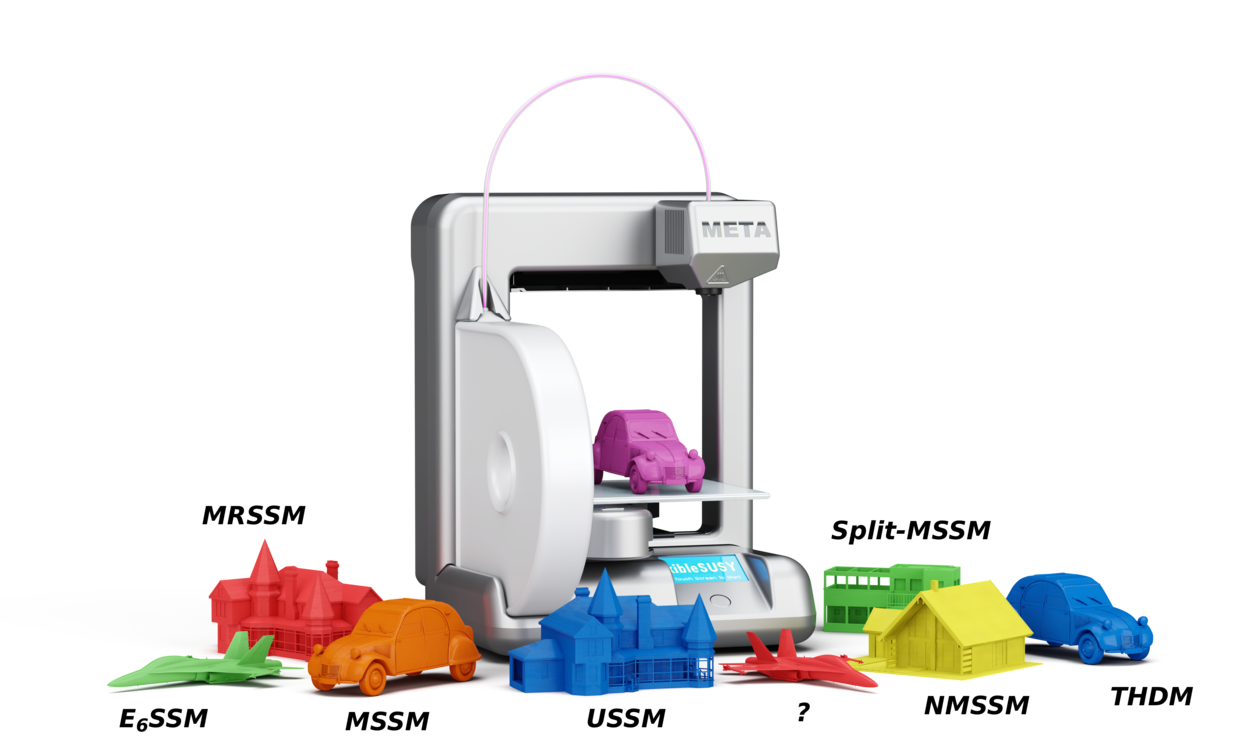
\includegraphics[width=\textwidth]{images/FS.png}
  \end{center}
\end{frame}

\begin{frame}{Generating a spectrum generator}
  \begin{figure}
    \centering
    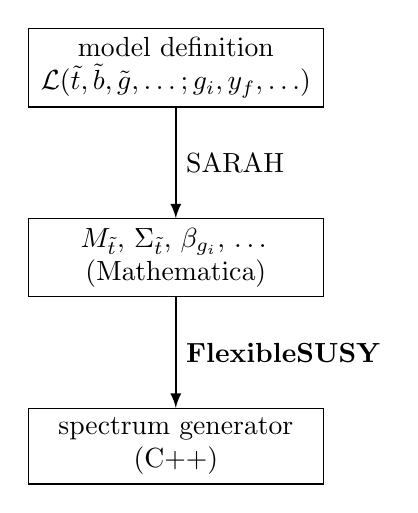
\begin{tikzpicture}[node distance=4em]
      \node [block, text width=10em] (Lagr) {model definition\\ $\Lagr(\tilde t, \tilde b, \tilde g,\ldots; g_i, y_f,\ldots)$};
      \node [block, below=of Lagr, text width=10em] (expr1) {$M_{\tilde t}$, $\Sigma_{\tilde t}$, $\beta_{g_i}$,
        \ldots\\ (Mathematica)};
      \node [block, below=of expr1, text width=10em] (flexiblesusy) {spectrum generator\\(C++)};
      \path [arrow] (Lagr) -- node[right] {SARAH} (expr1);
      \path [arrow] (expr1) -- node[right] {\emph{FlexibleSUSY}} (flexiblesusy);
    \end{tikzpicture}
  \end{figure}
\end{frame}

%%%%%%%%%%%%%%%%%%%%%%%%%%%%%%%%%%%%%%%%

\begin{frame}{Available models (selection)}
  \begin{table}
    \centering
    \begin{tabular}{llll}
      Model             & RGEs & \multicolumn{2}{l}{diagrammatic $M_h$ contributions} \\
      \midrule
      MSSM              & 3L   & \multicolumn{2}{l}{1L + 2L $O((\alpha_t + \alpha_b) \alpha_s + (\alpha_t + \alpha_b)^2)$} \\
      NMSSM             & 2L   & \multicolumn{2}{l}{1L + 2L $O((\alpha_t + \alpha_b) \alpha_s + (\alpha_t + \alpha_b)^2)$} \\
      USSM              & 2L   & \multicolumn{2}{l}{1L + 2L $O((\alpha_t + \alpha_b) \alpha_s + (\alpha_t + \alpha_b)^2)$} \\
      E$_6$SSM          & 2L   & \multicolumn{2}{l}{1L + 2L $O((\alpha_t + \alpha_b) \alpha_s + (\alpha_t + \alpha_b)^2)$} \\
      THDM              & 2L   & 1L \\
      THDM + $\tilde{h}_i$ & 2L   & 1L \\
      THDM + split      & 2L   & 1L \\
    \end{tabular}
  \end{table}
\end{frame}

%%%%%%%%%%%%%%%%%%%%%%%%%%%%%%%%%%%%%%%%

\begin{frame}{Available models matched to the MSSM at $M_S$}
  \resizebox{\textwidth}{!}{%
    \begin{tabular}{llll}
      Model             & RGEs & diagrammatic $M_h$ & matching \\
                        &      & contributions      & conditions \\
      \midrule
      SM + split        & 2L   & 1L + 2L $O(\alpha_t (\alpha_s + \alpha_t))$       & 1L $\tilde{g}_{ij}$ $O(\alpha_t + \alpha_i)$ \\
      (SplitMSSM)       &      & \phantom{1L} + 3L gluino $O(\alpha_t \alpha_s^2)$ & + 1L $\lambda$ $O((\alpha_t + \alpha_i)^2)$ \\
                        &      &                                                  & + 2L $\lambda$ $O(\alpha_s \alpha_t^2)$ \\
                        &      &                                                  & \mycite{1407.4081} \\[0.5em]
      SM                & 3L   & 1L + 2L $O(\alpha_t (\alpha_s + \alpha_t))$ & 1L $\lambda$ $O((\alpha_t + \alpha_i)^2 + \alpha_b^2 + \alpha_\tau^2)$ \\
      (HSSUSY)          &      &                                            & + 2L $\lambda$ $O((\alpha_s + \alpha_t)\alpha_t^2)$ \\
                        &      &                                            & \mycite{1407.4081, 1504.05200} \\[0.5em]
      SM                & 3L   & 1L + 2L $O(\alpha_t (\alpha_s + \alpha_t))$ & 1L $\lambda$ + $O(p^2/M_S^2)$ terms \\
      (``mixed'')
    \end{tabular}}
\end{frame}

%%%%%%%%%%%%%%%%%%%%%%%%%%%%%%%%%%%%%%%%

\section{Approaches to predict $M_h$}

\begin{frame}{Approaches to predict $M_h$}
  \begin{minipage}[t]{0.45\textwidth}
    \centering
    Diagrammatic approach\\[1em]
    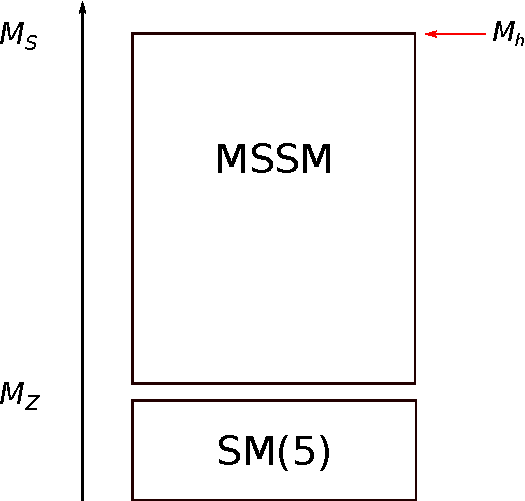
\includegraphics[width=\textwidth]{images/mssm-sm-tower-diagrammatic}
  \end{minipage}
  \hfill
  \begin{minipage}[t]{0.45\textwidth}
    \centering
    EFT approach\\[1em]
    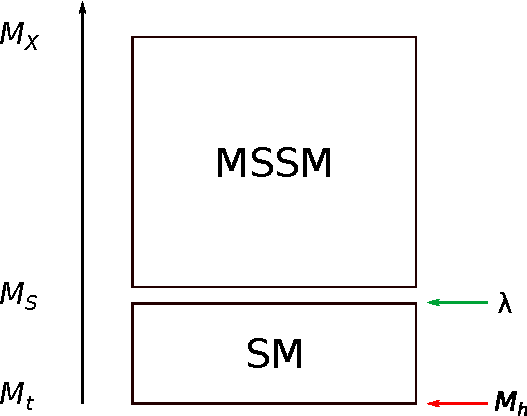
\includegraphics[width=\textwidth]{images/mssm-sm-tower-eft}
  \end{minipage}
\end{frame}

\begin{frame}{Diagrammatic approach (\DRbar\ codes)}
  \begin{center}
    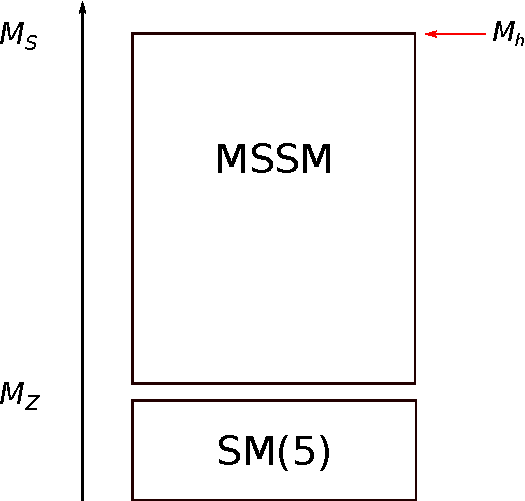
\includegraphics[width=0.45\textwidth]{images/mssm-sm-tower-diagrammatic}\\[1em]
  \end{center}
  \emph{Idea:} Calculate $M_h$ in the MSSM as a function of the \DRbar\ parameters:\\[1em]
  \centering $g_i$, $y^f_{ij}$, $v_i$, $\mu$, $B\mu$, $m^2_{H_i}$,
  $m_{\tilde{f},ij}^2$, $M_i$, $T^f_{ij}$
\end{frame}

\subsection{Diagrammatic approach}

\begin{frame}{Diagrammatic approach (\DRbar\ codes)}
  \emph{Fixed by observables:}
  \begin{table}
    \centering
    \begin{tabular}{lllll}
      Input & & & & Output \\
      \midrule
      $\alpha_\text{em}^{\SM(5)}(M_Z)$ & $\rightarrow$ & $\alpha_\text{em}^\MSSM(M_Z)$ & $\rightarrow$ & $g_1^\MSSM(M_Z)$ \\
      $G_F$ & $\rightarrow$ & $\sin\theta_W^\MSSM(M_Z)$ & $\rightarrow$ & $g_2^\MSSM(M_Z)$ \\
      $\alpha_\text{s}^{\SM(5)}(M_Z)$ & & & $\rightarrow$ & $g_3^\MSSM(M_Z)$ \\
      $M_Z$ & $\rightarrow$ & $m_Z^\MSSM(M_Z)$ & $\rightarrow$ & $v^\MSSM(M_Z)$ \\
      $M_t$ & $\rightarrow$ & $m_t^\MSSM(M_Z)$ & $\rightarrow$ & $y_t^\MSSM(M_Z)$ \\
      $m_b^{\SM(5)}(m_b)$ & $\rightarrow$ & $m_b^\MSSM(M_Z)$ & $\rightarrow$ & $y_b^\MSSM(M_Z)$ \\
      $M_\tau$ & $\rightarrow$ & $m_\tau^\MSSM(M_Z)$ & $\rightarrow$ & $y_\tau^\MSSM(M_Z)$ \\
    \end{tabular}
  \end{table}
  \emph{Fixed by 2 EWSB conditions:} $m^2_{H_u}$, $m^2_{H_d}$ \\[1em]
  \emph{Free parameters:} $\tan\beta$, $\mu$, $B\mu$, $m_{\tilde{f},ij}^2$, $M_i$,
  $T^f_{ij}$
\end{frame}

\begin{frame}{Diagrammatic approach (\DRbar\ codes)}
  \begin{align*}
    (M_h^\text{MSSM})^2 &= \text{smallest eigenvalue of} \\
    &\phantom{={}} \left[(m_h^\text{MSSM})^2 - \Sigma^\text{MSSM}_h(p^2 = (M_h^\text{MSSM})^2,Q = M_S)\right]_{ij}
  \end{align*}
  \emph{Advantage:} includes terms $O(p^2/M_S^2)$\\
  \emph{Disadvantage:} suffers from large logarithms $\propto\log(M_Z/M_S)$ if $M_S\gg M_Z$\\
\end{frame}

%%%%%%%%%%%%%%%%%%%%%%%%%%%%%%%%%%%%%%%%

\subsection{EFT approach}

\begin{frame}{EFT approach}
  \begin{center}
    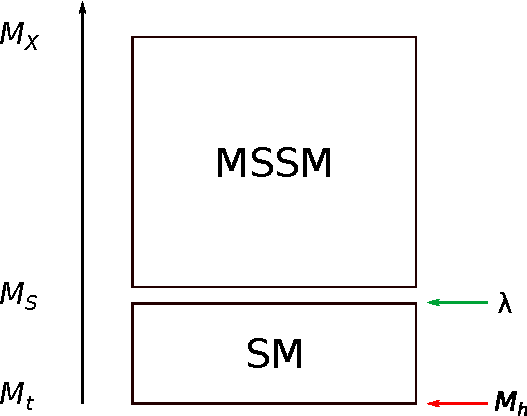
\includegraphics[width=0.45\textwidth]{images/mssm-sm-tower-eft}\\[1em]
  \end{center}
  \emph{Idea:} Calculate $M_h$ in the SM as a function of the \MSbar\ parameters:\\[1em]
  \centering $g_i$, $y^f_{ij}$, $v$, $\mu^2$, $\lambda$
\end{frame}

\begin{frame}{EFT approach}
  \emph{Fixed by observables:}
  \begin{table}
    \centering
    \begin{tabular}{lllll}
      Input & & & & Output \\
      \midrule
      $\alpha_\text{em}^{\SM(5)}(M_Z)$ & $\rightarrow$ & $\alpha_\text{em}^\SM(M_Z)$ & $\rightarrow$ & $g_1^\SM(M_Z)$ \\
      $G_F$ & $\rightarrow$ & $\sin\theta_W^\SM(M_Z)$ & $\rightarrow$ & $g_2^\SM(M_Z)$ \\
      $\alpha_\text{s}^{\SM(5)}(M_Z)$ & & & $\rightarrow$ & $g_3^\SM(M_Z)$ \\
      $M_Z$ & $\rightarrow$ & $m_Z^\SM(M_Z)$ & $\rightarrow$ & $v^\SM(M_Z)$ \\
      $M_t$ & $\rightarrow$ & $m_t^\SM(M_Z)$ & $\rightarrow$ & $y_t^\SM(M_Z)$ \\
      $m_b^{\SM(5)}(m_b)$ & $\rightarrow$ & $m_b^\SM(M_Z)$ & $\rightarrow$ & $y_b^\SM(M_Z)$ \\
      $M_\tau$ & $\rightarrow$ & $m_\tau^\SM(M_Z)$ & $\rightarrow$ & $y_\tau^\SM(M_Z)$ \\
    \end{tabular}
  \end{table}
  \emph{Fixed by 1 EWSB condition:} $\mu^2$ \\[1em]
  \emph{Free parameter:} $\lambda$
\end{frame}

\begin{frame}{EFT approach: matching all $\Gamma_{\phi_1,\ldots,\phi_n}$}
  Determine $\lambda(M_S)$ from mathching all $\Gamma_{\phi_1,\ldots,\phi_n}$:
  \begin{align*}
    \frac{\partial}{\partial p^2}\Gamma_{hh}^{\SM}(p^2 = 0, Q = M_S) &= \frac{\partial}{\partial p^2}\Gamma_{hh}^\text{MSSM}(p^2 = 0, Q = M_S) \\
    \Gamma_{hhhh}^{\SM}(p^2 = 0, Q = M_S) &= \Gamma_{hhhh}^\text{MSSM}(p^2 = 0, Q = M_S)
  \end{align*}
  $\Rightarrow$
  \begin{align*}
    \lambda (M_S) &= \frac{1}{4}\left[\frac{3}{5} g_1^{2} + g_2^2\right] \cos^22\beta
    + \Delta \lambda
  \end{align*}
  $\Rightarrow$
  \begin{align*}
    (M_h^\SM)^2 &= \lambda(M_Z) v^2(M_Z) - \Sigma^\SM_h(p^2 = (M_h^\SM)^2,Q =
    M_Z)
    % \\
    % &\phantom{={}} + t^\SM(Q=M_Z)
  \end{align*}
  \emph{Advantage:} resums large logarithms $\propto\log(M_Z/M_S)$\\
  \emph{Disadvantage:} neglects terms $O(p^2/M_S^2)$ from SUSY particles at 1L
\end{frame}

\begin{frame}{Comparison diagrammatic vs.\ EFT approach}
  \begin{figure}
    \centering
    \includegraphics[width=\textwidth]{plots/PlotScale-in-FH_new_low-notower}
  \end{figure}
  $\tan\beta = 5$, $X_{t,b,\tau} = 0$
\end{frame}

%%%%%%%%%%%%%%%%%%%%%%%%%%%%%%%%%%%%%%%%

\subsection{Mixed approach}

\begin{frame}{Combining EFT and diagrammatic approach}
  \begin{center}
    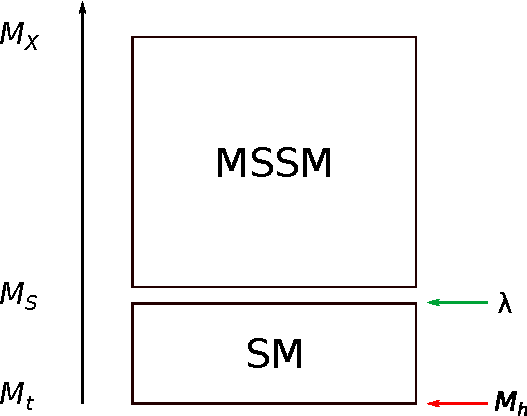
\includegraphics[width=0.45\textwidth]{images/mssm-sm-tower-eft}\\[1em]
  \end{center}
  \emph{Idea:} Calculate $M_h$ in the SM as a function of the \MSbar\ parameters:\\[1em]
  \begin{center}
    $g_i$, $y^f_{ij}$, $v$, $\mu^2$, $\lambda$
  \end{center}
  \emph{including terms $O(p^2/M_S^2)$ from SUSY particles at 1L}
\end{frame}

\begin{frame}{Combining EFT and diagrammatic approach: matching $M_h$}
  \begin{align*}
    M_h^{\SM} &\overset{!}{=} M_h^\text{MSSM} \quad \text{at} \quad Q = M_S
  \end{align*}
  $\Rightarrow$
  \begin{align*}
    \lambda(M_S) = \frac{1}{v^2(M_S)} \Big[
    {\color{normal text.fg!15!normal text.bg}
    \only<2->{\color{normal text.fg}}{%
    \underbrace{\usebeamercolor[fg]{text}{(M_h^\text{MSSM})^2 + \Sigma^\SM_h(p^2 = (M_h^\SM)^2,Q = M_S)}}_{\text{large logs $\propto\log(M_Z/M_S)$ cancel in SM limit}}}}
    \Big]
  \end{align*}
  where
  \begin{align*}
    (M_h^{\SM})^2 &= \lambda(M_S) v^2(M_S) - \Sigma^{\SM}_h(p^2 = (M_h^{\SM})^2,Q = M_S) \\
    (M_h^\text{MSSM})^2 &= \text{smallest eigenvalue of} \\
    &\phantom{={}} \left[(m_h^\text{MSSM})^2 - \Sigma^\text{MSSM}_h(p^2 = (M_h^\text{MSSM})^2,Q = M_S)\right]_{ij}
  \end{align*}
\end{frame}

\begin{frame}{Combining EFT and diagrammatic approach: matching $M_h$}
  Next step: RG running to $Q = M_Z$\\
  $\Rightarrow$
  \begin{align*}
    (M_h^{\SM})^2 &= \lambda(M_Z) v^2(M_Z) - \Sigma^{\SM}_h(p^2 = (M_h^{\SM})^2,Q = M_Z)
  \end{align*}
  \emph{Advantages:}
  \begin{itemize}
  \item includes 1L terms $O(p^2/M_S^2)$ from SUSY particles
  \item resums large logarithms $\log(M_Z/M_S)$ due to RG running
  \item incorporates SUSY particle mixings
  \item easily automatizable
  \end{itemize}
  \emph{Disadvantage:}
  \begin{itemize}
  \item large logs in matching cancel only in SM limit $\cos(\beta - \alpha) \rightarrow 0$
  \end{itemize}
\end{frame}

%%%%%%%%%%%%%%%%%%%%%%%%%%%%%%%%%%%%%%%%

\section{Comparison}

\begin{frame}{Comparison diagrammatic vs.\ EFT vs.\ mixed approach}
  \begin{figure}
    \centering
    \includegraphics[width=\textwidth]{plots/PlotScale-in-FH_new_low-selected}
  \end{figure}
  $\tan\beta = 5$, $X_{t,b,\tau} = 0$
\end{frame}

\begin{frame}{Comparison diagrammatic vs.\ EFT vs.\ mixed approach}
  \begin{figure}
    \centering
    \includegraphics[width=\textwidth]{plots/PlotScale-in-FH_new_low-selected-high}
  \end{figure}
  $\tan\beta = 5$, $X_{t,b,\tau} = 0$
\end{frame}

%%%%%%%%%%%%%%%%%%%%%%%%%%%%%%%%%%%%%%%%

\section{Equivalence of EFT and mixed approach}

\begin{frame}{Equivalence EFT and mixed approach $O(y_t^2)$}
  \begin{align*}
    M_h^{\SM} &\overset{!}{=} M_h^\text{MSSM} \quad \text{at} \quad Q = M_S
  \end{align*}
  where
  \begin{align*}
    (M_h^{\SM})^2 &= \lambda v^2 - \Sigma^{\SM}_h + t_h^\SM \\
    t_h^\SM &= -6 (y_t^\SM)^2 A_0(m_t)
  \intertext{and}
    (M_h^\MSSM)^2 &= \frac{1}{4} (g_Y^2 + g_2^2) v^2 c^2_{2\beta}
    - \Sigma_h^\MSSM + t_h^\MSSM\\
    \Sigma_h^\MSSM &= \Sigma_h^\SM \frac{c^2_\alpha}{s^2_\beta}
    + 3 (y_t^\SM)^2 \frac{c^2_\alpha}{s^2_\beta} \Big\{
       A_0(m_{Q_3}) + A_0(m_{U_3})\\
       &\phantom{={}} + 2 m_t \big[ B_0(m_{Q_3},m_{Q_3}) + B_0(m_{U_3},m_{U_3}) \big]
    \Big\}\\
    t_h^\MSSM &= -3 (y_t^\SM)^2 \frac{c^2_\alpha}{s^2_\beta} \Big[2 A_0(m_t) - A_0(m_{Q_3}) - A_0(m_{U_3})\Big]
  \end{align*}
\end{frame}

\begin{frame}{Equivalence EFT and mixed approach $O(y_t^2)$}
  in SM limit $\frac{c^2_\alpha}{s^2_\beta} \rightarrow 1$\\
  $\Rightarrow$ 
  \begin{align*}
    \lambda &= \frac{1}{4} (g_Y^2 + g_2^2) c_{2\beta}^2\\
    &\phantom{={}}
    - 3 (y_t^\SM)^4 \Big[
    B_0(p^2,m_{Q_3},m_{Q_3}) + B_0(p^2,m_{U_3},m_{U_3}) \Big]\\
    &=
    \frac{1}{4} (g_Y^2 + g_2^2) c_{2\beta}^2\\
    &\phantom{={}} - 3 (y_t^\SM)^4 \Big[
    -\log\frac{m^2_{Q_3}}{Q^2} + \frac{p^2}{6m^2_{Q_3}} + O\Big(\frac{p^4}{m^4_{Q_3}}\Big)\\
    &\phantom{={} - 3 (y_t^\SM)^4 \Big[}
    - \log\frac{m^2_{U_3}}{Q^2} + \frac{p^2}{6m^2_{U_3}} + O\Big(\frac{p^4}{m^4_{U_3}}\Big) \Big]\\
    &= [\text{Bagnaschi et.\ al. 2014}]
    + O\Big(\frac{p^2}{m^2_{Q_3}}\Big)
    + O\Big(\frac{p^2}{m^2_{U_3}}\Big)
  \end{align*}
\end{frame}

%%%%%%%%%%%%%%%%%%%%%%%%%%%%%%%%%%%%%%%%

\section{Summary}

\begin{frame}{Summary}
  \emph{Summary:}
  \begin{itemize}
  \item diagrammatic approach suffers from large logs $\propto\log(M_Z/M_S)$
  \item EFT approach misses terms $O(p^2/M_S^2)$ at 1L
  \item mixed approach
    \begin{itemize}
    \item includes terms $O(p^2/M_S^2)$ at 1L
    \item resums large logs $\propto\log(M_Z/M_S)$
    \item handles SUSY particle mixings
    \item can be automatized easily \emph{automatized} $\rightarrow$
      incorporation into FlexibleSUSY
    \item large logs cancel only in SM limit
    \end{itemize}
  \end{itemize}
  \emph{Todo:}
  \begin{itemize}
  \item matching $M_h$ at 2-loop level
  \end{itemize}
\end{frame}

%%%%%%%%%%%%%%%%%%%%%%%%%%%%%%%%%%%%%%%%
% backup slides
%%%%%%%%%%%%%%%%%%%%%%%%%%%%%%%%%%%%%%%%

\begin{frame}[noframenumbering]
  \begin{center}
    \Huge Backup
  \end{center}
\end{frame}

\begin{frame}[noframenumbering]{Comparison diagrammatic vs.\ EFT vs.\ mixed approach}
  \begin{figure}
    \centering
    \includegraphics[width=\textwidth]{plots/PlotScale-in-FH_new_low}
  \end{figure}
  $\tan\beta = 5$, $X_{t,b,\tau} = 0$
\end{frame}

% \begin{frame}[noframenumbering]{Comparison diagrammatic / EFT}
%   \begin{figure}
%     \centering
%     \includegraphics[width=\textwidth]{plots/PlotXt-selected}
%   \end{figure}
%   $\tan\beta = 5$, $X_{b,\tau} = 0$, $M_S = 2\eh{TeV}$
% \end{frame}

\begin{frame}[noframenumbering]{Calculation of $g_3^{\SM}(M_Z)$}
  \emph{Input:} \ \ $\alpha_{\text{s}}^{\SM(5)}(M_Z) = 0.1185$\\[1em]
  $\rightarrow$
  \begin{align*}
    \alpha_{\text{s}}^{\SM}(M_Z) &=
    \frac{\alpha_{\text{s}}^{\SM(5)}(M_Z)}{1 -
      \Delta\alpha_{\text{s}}(M_Z)} \intertext{with}
    \Delta\alpha_{\text{s}}(Q) &=
    \frac{\alpha_\text{s}}{2\pi} \left[
      -\frac{2}{3} \log{\frac{m_t}{Q}} \right]
    \intertext{$\Rightarrow$}
    g_{3}^{\SM}(M_Z) &=
    \sqrt{4\pi\alpha_{\text{s}}^{\SM}(M_Z)}
  \end{align*}
\end{frame}

\begin{frame}[noframenumbering]{Calculation of $y_t^{\SM}(M_Z)$}
  \begin{align*}
    y_t^{\SM}(M_Z) &= \frac{\sqrt{2}\, m_{t}^{\SM}(M_Z)}{v(M_Z)}
    %
    \intertext{where}
    %
    m_{t}^{\SM}(Q) &= M_t +
    \re\Sigma_{t}^{S}(M_Z) + M_t \Big[ \re\Sigma_{t}^{L}(M_Z) \\
    &\phantom{={}} +
    \re\Sigma_{t}^{R}(M_Z) + \Delta
    m_t^{1L,\text{gluon}} + \Delta m_t^{2L,\text{gluon}} \Big]\\
    % m_{t}^{\text{\MSbar}} &= M_t +
    % \Sigma_{t}^\text{no gluon}(M_Z) + M_t \Big[\Delta
    % m_t^{(1L),\text{gluon}} + \Delta m_t^{(2L),\text{gluon}} \Big]
    % \\
    \Delta m_t^{1L,\text{gluon}} &= -\frac{g_3^2}{12 \pi^2}
    \left[4 - 3 \log\left(\frac{m_t^2}{Q^2}\right)\right]
    \\
    \Delta m_t^{2L,\text{gluon}} &= \left(\Delta
      m_t^{1L,\text{gluon}}\right)^2 \\
    &\phantom{=\;} - \frac{g_3^4}{4608 \pi^4} \Bigg[396
    \log^2\left(\frac{m_t^2}{Q^2}\right)
    - 2028 \log\left(\frac{m_t^2}{Q^2}\right) \\
    &\phantom{=\; - \frac{g_3^4}{4608 \pi^4}\Bigg[} -48
    \zeta(3)+2821+16 \pi ^2 (1+\log 4)\Bigg]
  \end{align*}
  $\Rightarrow$
\end{frame}

\begin{frame}[noframenumbering]{Calculation of $v^\SM$}
  The VEV $v^\SM$ is calculated from the running $Z$ mass at $Q = M_Z$:
  \begin{align*}
    v^{\SM}(M_Z) &= \frac{2 m_Z^{\SM}(M_Z)}{\sqrt{g_Y^2 + g_2^2}} \\
    m_Z^{\SM}(M_Z) &= \sqrt{M_Z^2 + \Pi_Z^{1L}(p^2=M_Z^2,Q=M_Z)}
  \end{align*}
  $v^{\SM}$ evolves under RG running according to\\\bigcite{Sperling,
    Stöckinger, AV, 2013, 2014}
\end{frame}

\begin{frame}[noframenumbering]{Calculation of $g_3^\MSSM(M_S)$}
  \begin{align*}
    \alpha_{\text{s}}^{\MSSM}(M_S) &=
    \frac{\alpha_{\text{s}}^{\SM}(M_S)}{1 -
      \Delta\alpha_{\text{s}}(M_S)} \intertext{with}
    \Delta\alpha_{\text{s}}(Q) &= \frac{\alpha_\text{s}}{2\pi}\left[
      \frac{1}{2}-\sum_{\text{SUSY particle } f} T_f
      \log{\frac{m_f}{Q}} \right] \intertext{$\Rightarrow$}
    g_{3}^{\MSSM}(M_S) &= \sqrt{4\pi\alpha_{\text{s}}^{\MSSM}(M_S)}
  \end{align*}
\end{frame}

\begin{frame}[noframenumbering]{Calculation of $v_i^\MSSM(M_S)$}
  \begin{align*}
    M_Z^\SM = M_Z^\MSSM
  \end{align*}
  $\Rightarrow$
  \begin{align*}
    (m_Z^{\MSSM}(M_S))^2 &= (M_Z^\SM)^2 + \Pi_Z^{\MSSM,1L}(Q=M_S) \\
    (M_Z^{\SM})^2 &= \frac{1}{4} \left[(g_Y^\SM)^2 + (g_2^\SM)^2\right] (v^\SM)^2 - \Pi_Z^{\SM,1L}(Q=M_S)
  \end{align*}
  $\Rightarrow$
  \begin{align*}
    v^\MSSM(M_S) &= \frac{2 m_Z^{\MSSM}(M_S)}{\sqrt{(g_Y^\MSSM)^2 + (g_2^\MSSM)^2}}
    \intertext{$\Rightarrow$}
    v_u^{\MSSM}(M_S) &= v^\MSSM(M_S) \sin\beta(M_S) \\
    v_d^{\MSSM}(M_S) &= v^\MSSM(M_S) \cos\beta(M_S)
  \end{align*}
\end{frame}

\begin{frame}[noframenumbering]{Calculation of $y_i^\MSSM(M_S)$}
  \begin{align*}
    M_f^\SM = M_f^\MSSM
  \end{align*}
  $\Rightarrow$
  \begin{align*}
    m_f^{\MSSM}(M_S) &= M_f^\SM + \Sigma_f^{\MSSM,1L}(Q=M_S) \\
    M_f^{\SM} &= \frac{\sqrt{2} m_f^\SM}{v_i^\SM} - \Sigma_f^{\SM,1L}(Q=M_S)
  \end{align*}
  $\Rightarrow$
  \begin{align*}
    y_f^\MSSM(M_S) = \frac{\sqrt{2} m_f^\MSSM(M_S)}{v_i^\MSSM(M_S)}
  \end{align*}
\end{frame}

\begin{frame}[noframenumbering]{FlexibleSUSY's Weltanschauung}
  \begin{itemize} \setlength\itemsep{2em}
  \item Model is defined in terms of Lagrangian parameters:\\
    $g_i$, $y_{ij}$, $v_i$, \ldots in the \MSbar/\DRbar\ scheme
  \item Input parameters:\\
    $\alpha_{\text{em},\text{SM}}^{(5),\MSbar}(M_Z)$,
    $\alpha_{\text{s},\text{SM}}^{(5),\text{\MSbar}}(M_Z)$, $M_Z$,
    $M_t$, $G_F$, \ldots
  \item Output parameters:\\ $m_h$, $M_h$, \ldots
  \end{itemize}
\end{frame}

\begin{frame}[noframenumbering]{Physical problem statement for the SM}
  \begin{figure}[tbh]
    \centering
    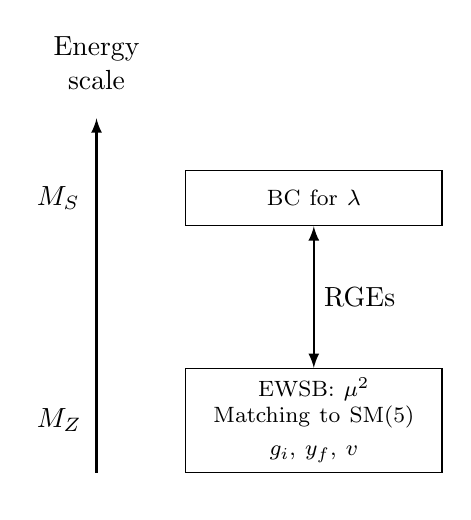
\begin{tikzpicture}[node distance = 3.5cm, auto]
      \node [block, text width=8.6em] (lowscale) {\footnotesize EWSB: $\mu^2$\\ Matching to SM(5)\\ $g_i$, $y_f$, $v$};
      \node [block, above=1.8cm of lowscale, text width=8.6em] (highscale) {\footnotesize BC for $\lambda$};
      \path [arrow2] (highscale) -- node {RGEs} (lowscale);
      % energy axis
      \node [below left=0em and 1cm of lowscale] (energy_start) {};
      \node [above=4.5cm of energy_start] (energy_stop) {};
      \node [above=0em of energy_stop,align=center] (energy_label) {Energy \\ scale};
      \path [arrow] (energy_start) -- (energy_stop);
      \node [text width=2em,left=3.0em of highscale] (mx) {$M_S$};
      \node [text width=2em,left=3.0em of lowscale] (mz) {$M_Z$};
    \end{tikzpicture}
  \end{figure}
\end{frame}

\begin{frame}[noframenumbering]{Algorithm to calculate the model parameters consistent with all BCs}
  \begin{figure}[tbh]
    \centering
    \small
    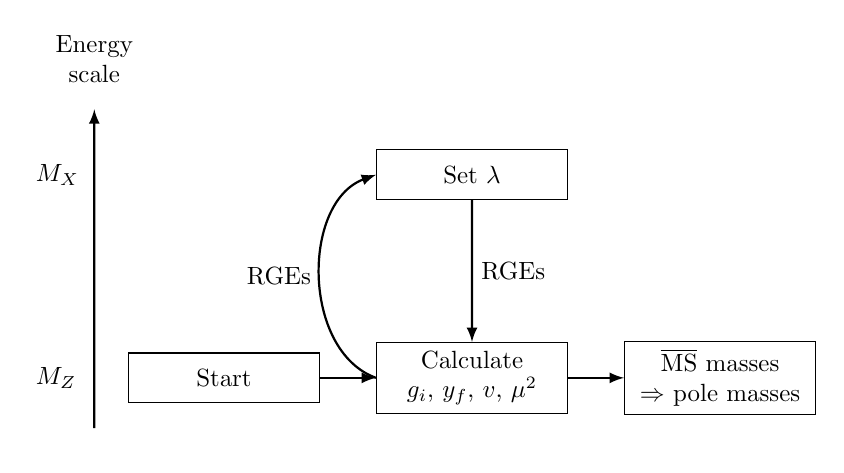
\begin{tikzpicture}[node distance = 3.5cm, auto,scale=0.9, every node/.style={transform shape}]
      \node [block] (guess) {Start};
      \node [block, right of=guess] (lowscale) {Calculate\\ $g_i$, $y_f$, $v$, $\mu^2$};
      \node [block, above=2cm of lowscale] (highscale) {Set $\lambda$};
      \node [block, right of=lowscale] (spec) {\MSbar\ masses\\ $\Rightarrow$ pole masses};
      \path [arrow] (guess) -- (lowscale);
      \path [-latex, thick] (lowscale.west) edge[bend left=70] node {RGEs} (highscale.west);
      \path [arrow] (highscale) -- node {RGEs} (lowscale);
      \path [arrow] (lowscale) -- (spec);
      % energy axis
      \node [below left=1em and 1em of guess] (energy_start) {};
      \node [above=4.5cm of energy_start] (energy_stop) {};
      \node [above=0em of energy_stop,align=center] (energy_label) {Energy\\ scale};
      \path [arrow] (energy_start) -- (energy_stop);
      \node [text width=3.3em,left=10em of highscale] (mx) {$M_X$};
      \node [text width=3.3em,left=10em of lowscale] (mz) {$M_Z$};
    \end{tikzpicture}
  \end{figure}
\end{frame}

\end{document}
